\documentclass[12pt]{article}
\usepackage{graphicx}
\usepackage{subcaption}
\usepackage{hyperref}
\usepackage{bookmark}
\usepackage{geometry}
\usepackage{color}
\usepackage{listings}
\usepackage{caption}
\usepackage{fancyhdr}
\usepackage{amsmath}
\usepackage{upquote}
\usepackage{array}
\usepackage{float}


\geometry{margin=1in}
\pagestyle{fancy}
\fancyhf{}
\rhead{Chicago Crime ETL Pipeline}
\lhead{Nishan Khanal}
\rfoot{\thepage}

\title{Chicago Crime Data ETL Pipeline Project}
\author{Nishan Khanal}
\date{\today}

\begin{document}

\maketitle

\tableofcontents

\newpage
\begin{abstract}
    This report describes the disign developement and deployment of a fully automated ETL pipeline orchestrated using Airflow to aid in the analysis and visualization of the Chicago crime dataset. The pipeline is designed to be lightweight, and fault tolorent - ready to be deployed in a prdocution envrironment. It integrates various components including extracting data from the official Chicago open data API, applying different transformations to clean and standardize the data, enriching it with spatial context (i.e., missing community areas), and loading the processed data efficiently into a PostgreSQL database hosted on Aiven (DigitalOcean). It is deployed on a Google Cloud micro VM (e2-micro instance) to ensure persistent, cloud-based data availability independent of local or VM storage with a robust logging and monitoring mechanism.
    \end{abstract}
    

\section{Introduction}

Crime prediction and public safety analysis rely heavily on clean, timely, and spatially accurate data. This project aims to make that process easir by automating the ETL (Extract, Transform, Load) pipeline for the Chicago Crime dataset. It fouses on periodically fetching the latest crime data from the Chicogo's official data api, cleaning and standardizing it, enriching the data with spatial context (i.e., missing community areas), and storing the processed data in a reliable, queryable cloud database. The pipeline is designed to be lightweight, fault-tolerant, and ready for production deployment.
he goal is to create a system that can continuously fetch the latest crime reports from Chicago's official data portal, clean and standardize them, enrich the data with spatial context (i.e., missing community areas), and store the processed data in a reliable, queryable cloud database.

This project focuses on setting up an ETL pipeline that can continuously fetch the latest crime reports from Chicago's official data portal, clean and standardize them, enrich the data with spatial context (i.e., missing community areas), and store the processed data in a reliable, queryable cloud database.
\subsection*{Dataset Choice}
Based on my proposal I've built the ETL pipeline for the \textbf{Chicago Crime dataset}. This dataset contains the reported incidents of crime in the City of Chicago from 2001 to present (minus the most recent 7 days). The dataset is deidentified in the spatial domain, i.e, the addresses are only accurate to the block level. This dataset will be helpful for analyzing crime patterns, and trends, and for predicting future crime hotspot. It is available in the official Chicago open data portal \href{https://data.cityofchicago.org/Public-Safety/Crimes-2001-to-Present/ijzp-q8t2}{here}. The dataset is updated daily, and the API allows for incremental updates, making it ideal for a continuous ETL pipeline.


A supplementary dataset \textbf{Chicago Community Areas} was also used which aided in the visualization of the crime location in different communities. This dataset contains geographic information (GIS) about the different communities in Chicago. This dataset is available in the official Chicago open data portal \href{https://data.cityofchicago.org/Community-Areas/Community-Areas-GeoJSON/4ykn-5ajh}{here}. This dataset was also used to impute the missing community area values in the crime dataset.


The core goals of this project were:
\begin{itemize}
\item To automate the end-to-end ETL process without manual intervention
\item To optimize the pipeline for execution on limited infrastructure (micro VM)
\item To decouple the pipeline from local resources for availability and maintainability
\item To ensure scalability, observability, and auditability in real-world conditions
\end{itemize}

Throughout this document, each component of the system will be described in detail, along with rationale, challenges, and architectural decisions made along the way.

\section{Technology Stack}

\subsection*{Languages and Frameworks}
\begin{itemize}
\item Python 3.10
\item Apache Airflow (version 2.7.2)
\item Pandas, GeoPandas, sodapy , Psycopg2
\item PostgreSQL (Aiven Free Tier)
\end{itemize}

\subsection*{Infrastructure}
\begin{itemize}
\item Google Cloud VM (e2-micro) running Ubuntu
\item Aiven PostgreSQL database (hosted on DigitalOcean)
\item GitHub for version control. (\href{https://github.com/nishanKhanal/e2e-data-pipeline-for-chicago-crime}{Link})
\end{itemize}

\subsection*{Development Tools}
\begin{itemize}
\item VS Code for development and SSH access
\item Tmux for persistent process handling on the VM
\item Systemd for automating Airflow as a background service
\end{itemize}

\section{Project Motivation and Planning}

Initially, I began working with the dataset on my local machine. I used \texttt{ngrok} to tunnel my PostgreSQL port and connect external services (like Google Looker Studio) for demo purposes. While this worked, it was not suitable for a long-running, always-on pipeline:

\begin{itemize}
\item \textbf{Ngrok is ideal for development}, but the connection times out frequently unless you're on a paid plan.
\item Relying on a \textbf{local database} meant the pipeline couldn't run unless my laptop was powered and connected.
\end{itemize}

To overcome this, I migrated to a \textbf{Google Cloud micro VM (e2-micro)} — a lightweight and cost-effective instance — to host my Airflow-based pipeline. I also moved my database to \textbf{Aiven's free-tier PostgreSQL instance (hosted on DigitalOcean)} to ensure persistent, cloud-based data availability independent of local or VM storage.

\section{Airflow Automation and Orchestration}

Airflow was chosen to automate and orchestrate the pipeline due to its flexibility, native scheduling, and observability features. Tasks are defined as Python callables, and dependencies are managed explicitly. The DAG consists of three tasks — \texttt{extract}, \texttt{transform}, and \texttt{load} — each executing the respective Python functions.

\subsection*{Airflow DAG Design}
The DAG is scheduled to run daily. A simple linear dependency is enforced: \texttt{extract} \textrightarrow{} \texttt{transform} \textrightarrow{} \texttt{load}.

% \begin{figure}[h!]
% \centering
% Replace with an actual screenshot of your DAG view
% \includegraphics[width=0.9\textwidth]{figures/airflow_dag_view.png}
% \caption{Airflow DAG visual showing extract-transform-load flow. \textit{(Include a screenshot from the Airflow UI DAG Graph View)}}
% \label{fig:dag_view}
% \end{figure}

\subsection*{Systemd Automation}
To ensure Airflow runs continuously without manual intervention, a systemd service was created to launch the scheduler and webserver in the background when the VM boots.

\begin{figure}[h!]
\centering
\begin{subfigure}{0.8\textwidth}
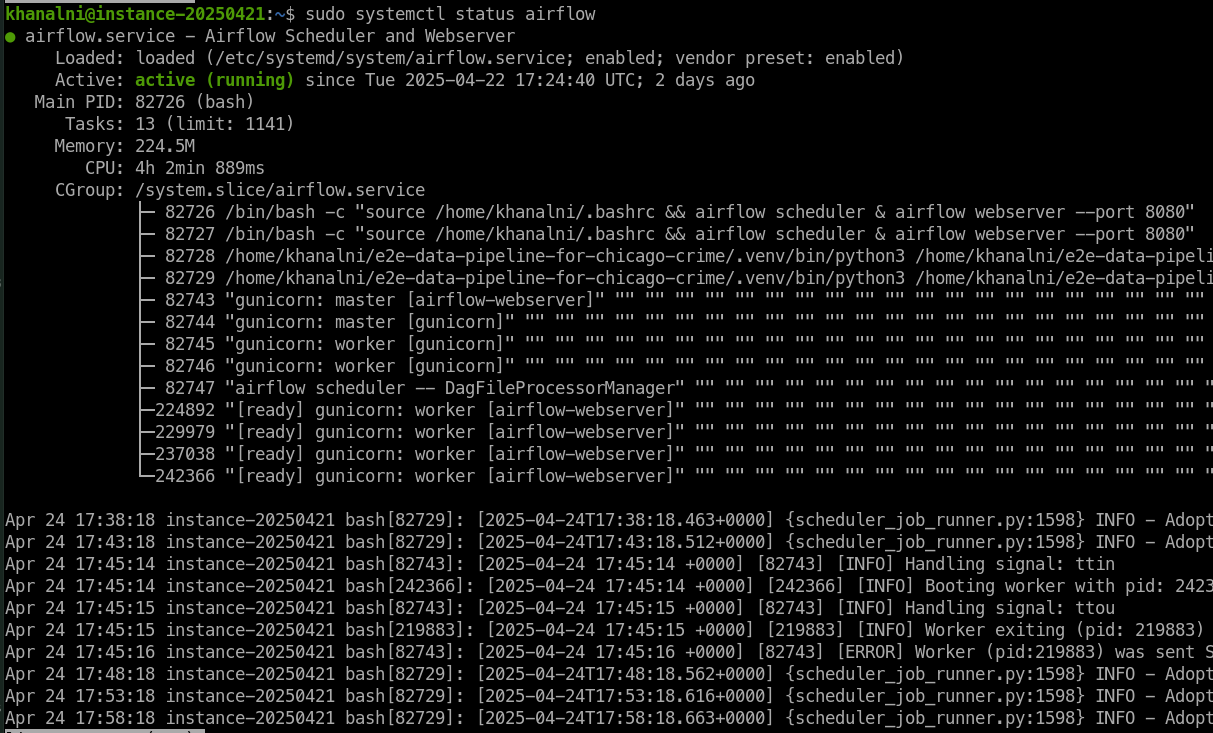
\includegraphics[width=\textwidth]{figures/systemd_status_airflow.png}
\caption{Systemd service status for Airflow}
\end{subfigure}
\hfill
% \begin{subfigure}{0.48\textwidth}
% \includegraphics[width=\textwidth]{figures/tmux_running_airflow.png}
% \caption{Airflow running inside Tmux session}
% \end{subfigure}
\caption{Automation of background execution using systemd}
\label{fig:systemd}
\end{figure}


\section{Pipeline Overview}

Figure \ref{fig:workflow} shows the ETL workflow. The data will be extracted from the Chicago Crime dataset and the Chicago Community Areas dataset. The data was be transformed through cleaning, normalization, enrichment, and data type conversion. The transformed data was then loaded into a PostgreSQL database hosted on Aiven. Finally, the data was be analyzed and visualized using Python libraries and GCP Looker Studio.

Figure \ref{fig:airflow_etl} shows the Airflow DAG for the ETL pipeline. The DAG is scheduled to run daily, and it consists of three tasks: \texttt{extract}, \texttt{transform}, and \texttt{load}. Each task is defined as a Python callable.
\begin{figure}[h!]
    \centering
    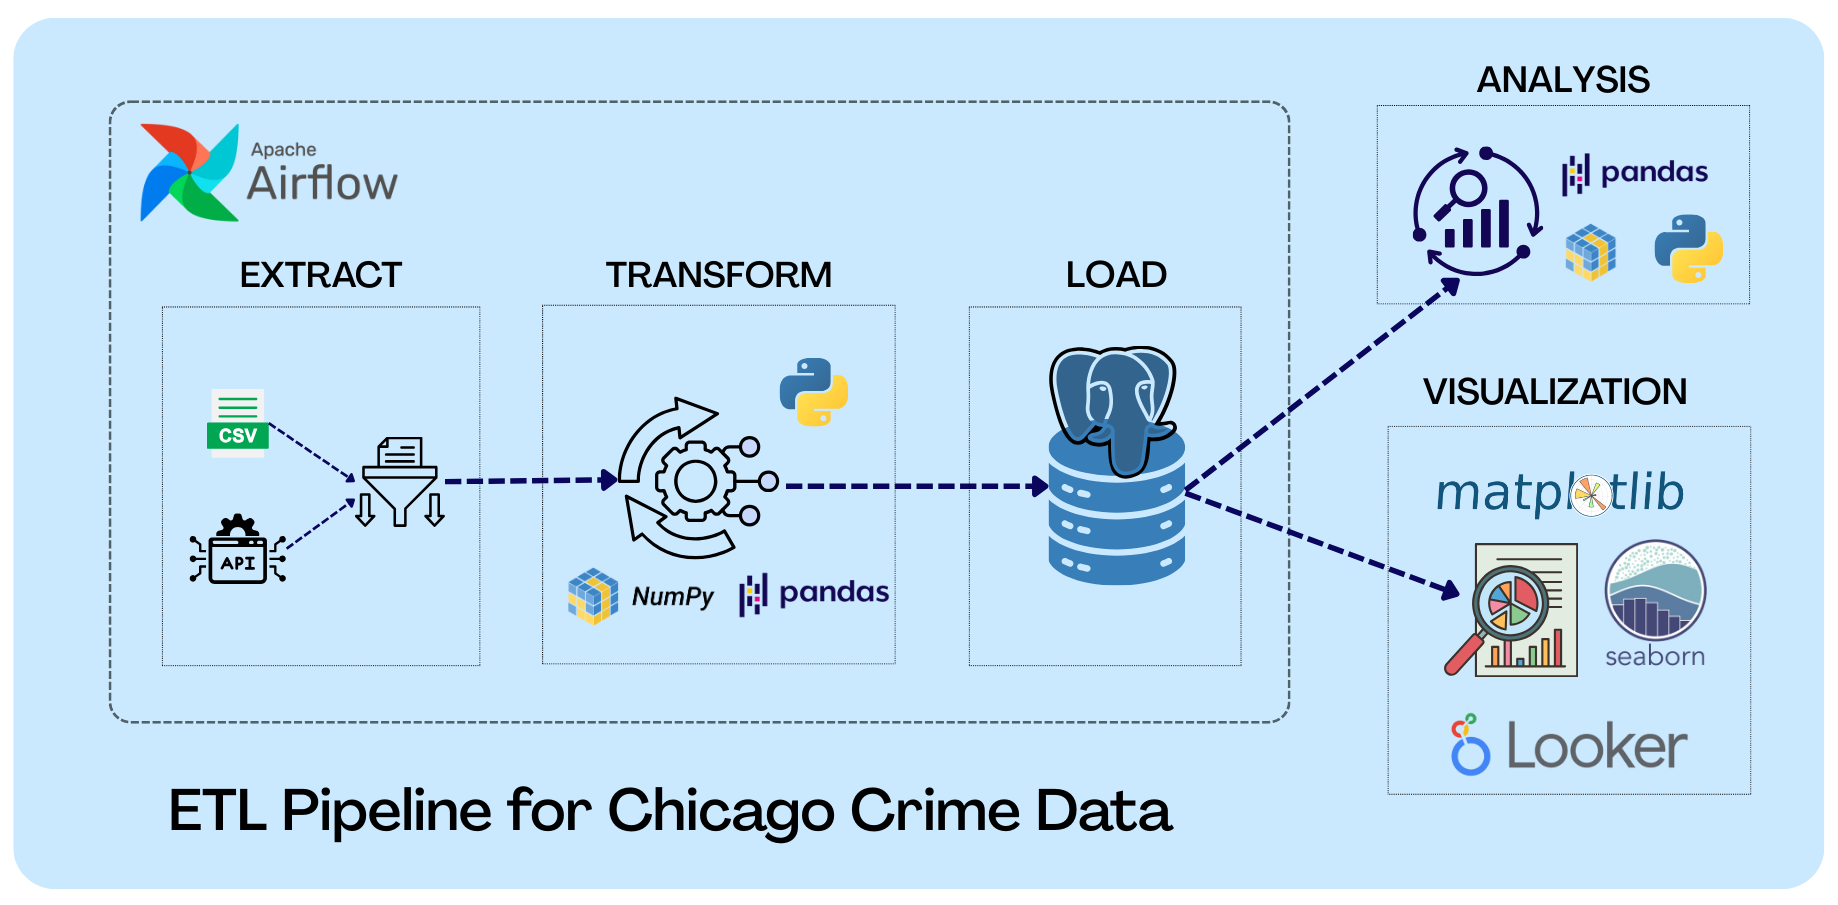
\includegraphics[width=1\textwidth]{figures/workflow.png}
    \caption{ETL Workflow}
    \label{fig:workflow}
\end{figure}

\begin{figure}[h!]
    \centering
    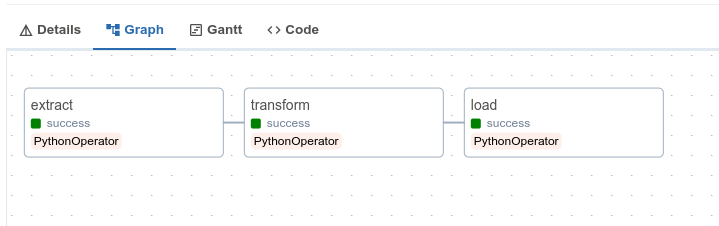
\includegraphics[width=1\textwidth]{figures/airflow_etl.png}
    \caption{Airflow DAG for ETL pipeline}
    \label{fig:airflow_etl}
\end{figure}



\section{Data Extraction}

The \texttt{extract()} function is the first step in the ETL pipeline. Its responsibility is to connect to the Socrata Open Data API hosted by the City of Chicago, retrieve all crime records that have been added or updated since the last successful load, and return them in memory as a list of dictionaries as shown in figure \ref{fig:extract_output}. Figure \ref{fig:extract_output} shows the logs of the extract phase with its successfull completion.

\subsection*{API Integration with Socrata}
The City of Chicago crime dataset is accessible via an open data API. This function authenticates using an application token and sends paginated requests, each limited to a batch size (default: 1000). A retry mechanism with \textbf{exponential backoff} ensures fault tolerance in the event of timeouts or transient network errors.


% \begin{figure}[h!]
%     \centering
%     \begin{subfigure}[t]{0.49\textwidth}
%         \centering
%         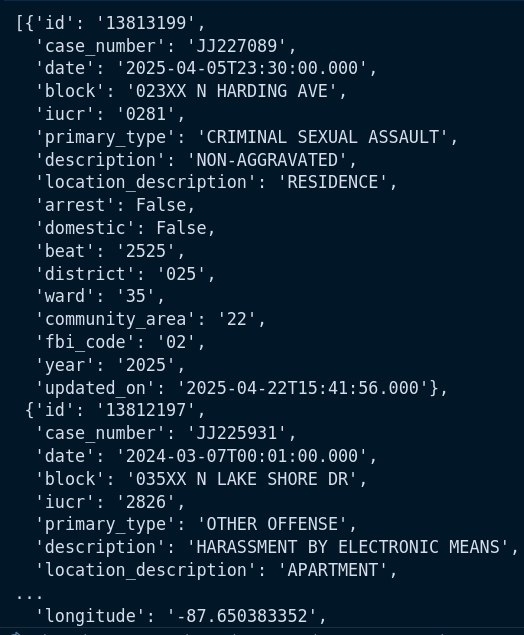
\includegraphics[width=\textwidth]{figures/extract_output.png}
%         \caption{Output of the extract phase}
%         \label{fig:extract_output}
%     \end{subfigure}\hfill
%     \begin{subfigure}[t]{0.49\textwidth}
%         \centering
%         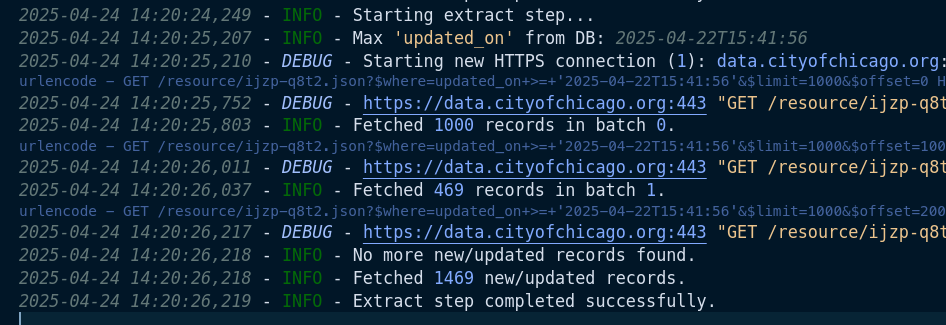
\includegraphics[width=\textwidth]{figures/extract_logs.png}
%         \caption{Logs of the extract phase}
%         \label{fig:extract_logs}
%     \end{subfigure}
%     \caption{Extract phase output and logs side by side}
%     \label{fig:extract_phase}
% \end{figure}

\begin{figure}[h!]
    \centering
    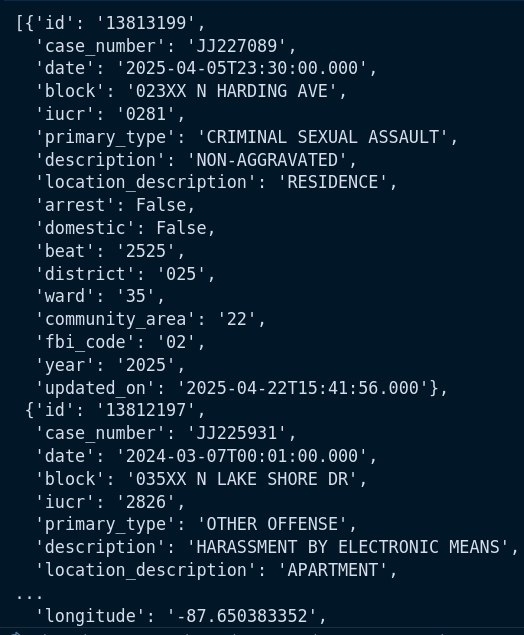
\includegraphics[width=0.5\textwidth]{figures/extract_output.png}
    \caption{Output of the extract phase}
    \label{fig:extract_output}
\end{figure}


\begin{figure}[H]
    \centering
    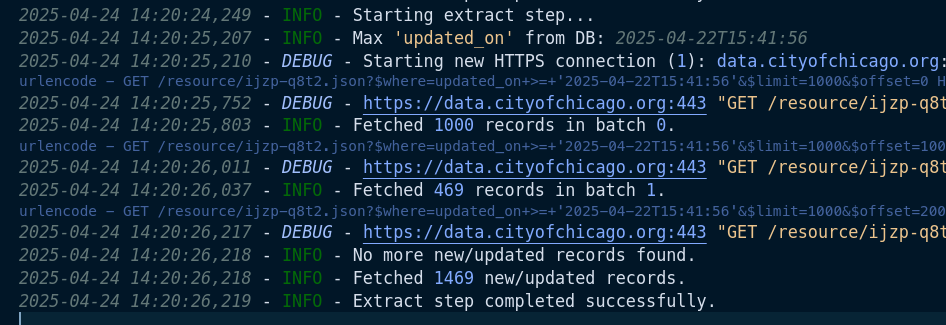
\includegraphics[width=0.9\textwidth]{figures/extract_logs.png}
    \caption{logs of the extract phase after of successfull execution}
    \label{fig:extract_logs}
\end{figure}


\subsection*{Tracking Incremental Updates}
To avoid re-fetching already-processed data, the extractor first queries the PostgreSQL database to find the maximum \texttt{updated\_on} timestamp in the \texttt{crimes} table. This value is used in a \texttt{WHERE} clause to fetch only new or modified records.

\subsection*{Error Handling}
The function includes structured exception handling. The logs generated by retry logic is also demonstrated in figure\ref{fig:extract_logs_exception}:
\begin{itemize}
    \item Raises \texttt{RuntimeError} if database connection fails or returns an invalid timestamp
    \item Raises \texttt{RuntimeError} if the API client fails to initialize
    \item Raises \texttt{RuntimeError} if retry limit is reached during a batch request
    \item Raises \texttt{ValueError} if no data is returned (indicating a possible upstream issue)
\end{itemize}

\begin{figure}[h!]
    \centering
    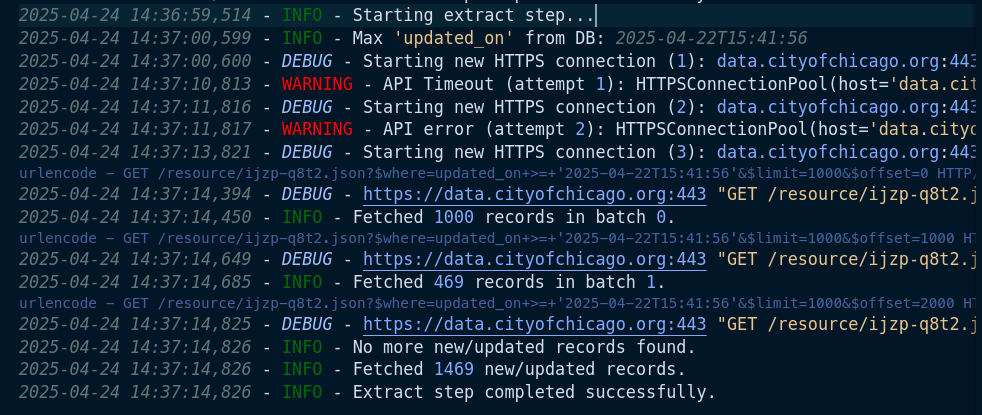
\includegraphics[width=0.9\textwidth]{figures/extract_logs_exception.png}
    \caption{Demonstration of system behavior during timeouts and transient n/w failure}
    \label{fig:extract_logs_exception}
\end{figure}


\subsection*{Design Decisions}
\begin{itemize}
    \item Raising exceptions (instead of returning empty lists) ensures that Airflow correctly marks the task as failed
    \item Pagination and retry logic are encapsulated in a nested \texttt{fetch\_with\_retry()} function for clarity and reuse. Pagination can also be seen on figure \ref{fig:extract_logs} with the first page fetching 1000 records and the second page fetching 469 records.
    \item Logs are written for each API call and each critical step, including retry attempts and batch sizes
\end{itemize}

\section{Data Transformation}

The \texttt{transform()} function is utilized to convert raw API data into clean, enriched,and structured form to be loaded into the database. This stage comprises rigorous datacleaning, standardization, and geospatial enrichment.

\subsection*{Input Validation and Schema Enforcement}
The function first validates the structure of the input \texttt{DataFrame}. If the DataFrame is empty or \texttt{None}, it raises a \texttt{ValueError}, immediately halting the DAG. After that, it ensures all the expected columns are present in the data frame. Then only the columns that are present in the database schema are selected, which is defined by the expected columns

\subsection*{Data Type Casting}
To enforce consistency and avoid downstream type mismatch errors, the function calls \texttt{cast\_column\_types()}, which converts each column to a specific type:
\begin{itemize}
    \item \texttt{Int64} for primary identifiers and codes
    \item \texttt{Float64} for coordinates
    \item \texttt{string} for categorical fields
    \item \texttt{boolean} for flags like \texttt{arrest} and \texttt{domestic}
    \item \texttt{datetime64[ns]} for \texttt{date} and \texttt{updated\_on}
\end{itemize}

\subsection*{String Normalization}
For all the string columns, leading/trainling whitespaces are stripped off, internal whitespaces are collapsed using regex and finally are converted to uppercase. This ensures uniform grouping and filtering duing the analytics and visualization phase. 

\subsection*{Spatial Imputation of Missing Community Areas}
Some records lack the \texttt{community\_area} field, which is critical for geographic analysis if we are to consider community areas as nodes for feeding the data to a graph nerural network. These are imputed based on the crime's \texttt{x\_coordinate} and \texttt{y\_coordinate} using a geospatial join with a geojson file of Chicago’s community area boundaries. If the location of a crime inciddent falls inside the area of a community area, it's \texttt{community\_area} attribute is imputed using the Community Area it falls inside. For example, in figure \ref{fig:imputation_example}, we can see that the crime incident with \texttt{case\_number}=\texttt{JJ219799} falls inside the community area \texttt{51}, sot its \texttt{community\_area} attribute is set as \texttt{51} 

\begin{figure}[h!]
    \centering
    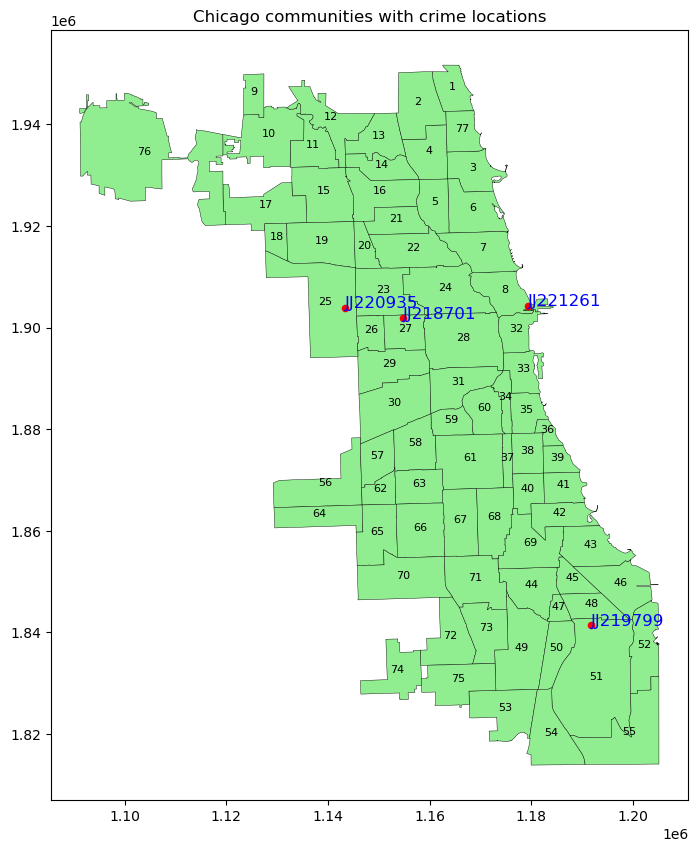
\includegraphics[width=0.9\textwidth]{figures/imputation_example.png}
    \caption{Demonstration of \texttt{community\_area} imputation}
    \label{fig:imputation_example}
\end{figure}


\subsection*{Row Cleaning and Deduplication}
The function removes rows based on configurable rules. For now, the function can remove all the rows for which any of the specified columns(drop\_if\_any\_null\_columns) have missing values, and all the rows for which all the values in the specified columns(drop\_if\_all\_null\_columns) are missing:
\begin{itemize}
    \item Drops rows with missing values in critical columns (optional logic)
    \item Drops rows where all coordinate fields are missing
    \item Deduplicates based on all columns except \texttt{id}
\end{itemize}

Dropped rows are saved to audit files named \texttt{audit\_missing\_drops\_\{timestamp\}.csv} and \texttt{audit\_duplicate\_drops\_\{timestamp\}.csv}, making the cleaning process fully transparent and reversible.

In figure \ref{fig:transform_output}, we can see the output of the transform fucntion for a select group of columns. Only these columns were included in the figure due to the space constraint. Here, we can see that, for some rows, latitude and longitude columns have missing values even after transformation; this is by design. Although the code to remove rows based on missing values of specific columns is present, I didn't specify any columns to check for null values for this task because these rows can still be important in the downstream task because they have the non-null values for other spatial columns like community\_area, beat, district, etc.

\begin{figure}[h!]
    \centering
    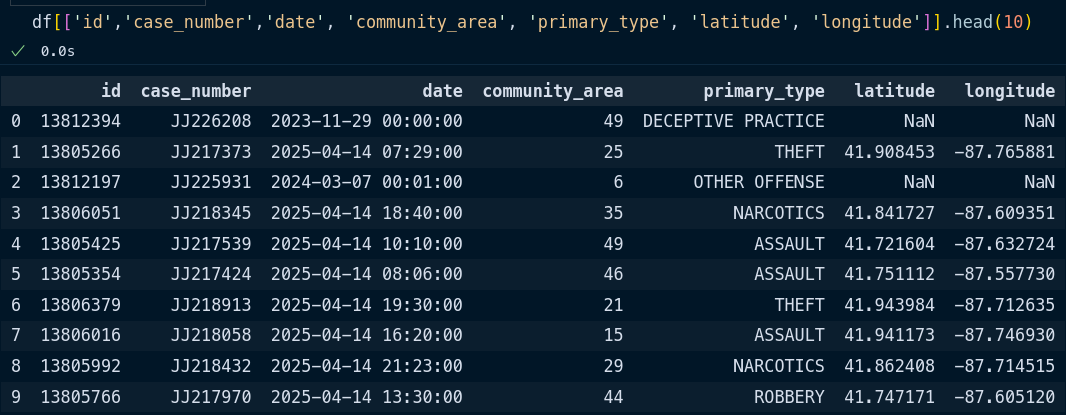
\includegraphics[width=0.9\textwidth]{figures/transformation_output.png}
    \caption{Output of the transform function}
    \label{fig:transform_output}
\end{figure}

\begin{figure}[h!]
    \centering
    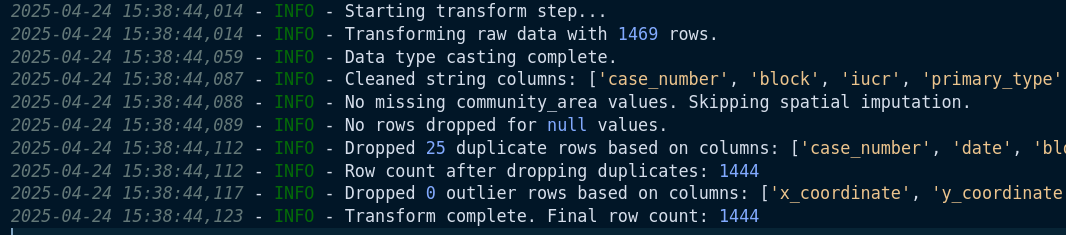
\includegraphics[width=0.9\textwidth]{figures/transform_logs.png}
    \caption{Logs generated by the transform function}
    \label{fig:transform_logs}
\end{figure}


\subsection*{Final Checks}
If all rows are dropped during the cleaning process, the function raises a \texttt{ValueError}, which signals Airflow to halt the DAG. Otherwise, it logs the final row count as shown in figure \ref{fig:transform_logs} and returns the cleaned DataFrame for loading.




\section{Data Loading}

The \texttt{load()} function performs the final step in the ETL pipeline: inserting the cleaned and transformed data into the PostgreSQL database hosted on Aiven. Since, I used this function to load both the continuous data from api and the historical data (which is massive with ~ 8 million rows), the function was optimised for bulk inserts at the same time supporting UPSERT behavior to ensure that the existing records are updated rather than duplicated.

\subsection*{Preparation for Insertion}
Before insertion, the function converts all null-like values (e.g., \texttt{pd.NA}, \texttt{NaN}) to Python-native \texttt{None} values using the helper function \texttt{prepare\_for\_postgres\_insertion()}. This avoids type mismatches when communicating with the database driver.

\subsection*{Conflict Detection}
To log how many rows will be inserted versus updated, the function queries the destination table for all existing \texttt{id} values in the current batch. It compares this list against the incoming data to log the following as shown in figure \ref{fig:load_log}:
\begin{itemize}
    \item Number of records that will be inserted (new)
    \item Number of records that will be updated (conflicts)
\end{itemize}

\begin{figure}[h!]
    \centering
    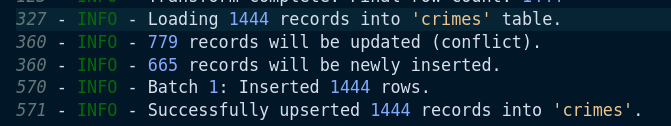
\includegraphics[width=0.9\textwidth]{figures/load_logs.png}
    \caption{Log output showing insert vs. update count}
    \label{fig:load_log}
\end{figure}

\subsection*{Batching and Performance}
The function uses \texttt{psycopg2.extras.execute\_values()} to insert data in batches (default: 50,000 rows per batch). This approach is significantly faster than inserting rows individually.

If a batch fails, it is rolled back and written to a CSV file named
\texttt{failed\_batch\_\{n\}\_\{timestamp\}.csv} for later inspection or reprocessing.

\subsection*{Error Handling and Robustness}
The function raises exceptions under the following conditions:
\begin{itemize}
    \item Failure to connect to the database
    \item Failure in all batches (complete load failure)
    \item Partial load success (some batches failed): a \texttt{RuntimeError} is raised after successful ones are committed, signaling Airflow while preserving inserted data
\end{itemize}

\begin{figure}[h!]
    \centering
    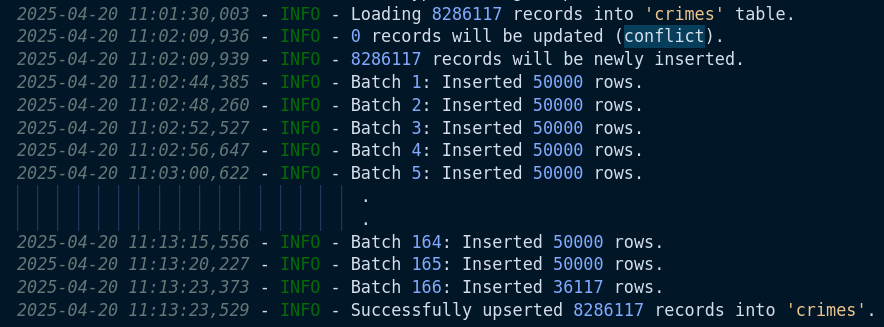
\includegraphics[width=0.9\textwidth]{figures/load_logs_batched.png}
    \caption{Log output showing multiple batch insert for historical data}
    \label{fig:load_log_batched}
\end{figure}

Figure \ref{fig:load_log_batched} show the logs of loading the entire historical crime data using the load() function. This shows that the function is capable of loading not only the data from the api but also huge historical data. I've manually trancated the logs to show only the first and last few batches.

\subsection*{Post-Load Outcome}
If at least one batch succeeds, the function logs the total number of records inserted and updated as shown in figure \ref{fig:load_log}, and returns cleanly. This enables downstream systems (e.g., dashboards or reports) to use the updated data immediately after load completion.

Figure \ref{fig:db_before_load} shows the crime incidents orderd by date column for a select few columns before the latest load() operation and figure \ref{fig:db_after_load} shows the crime incidents after the latest load() operation.

\begin{figure}[h!]
    \centering
    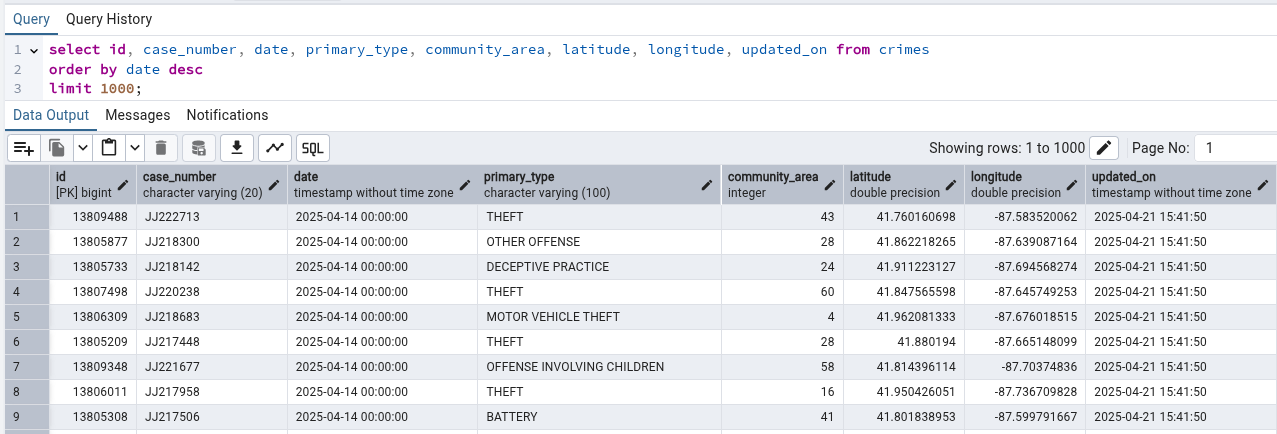
\includegraphics[width=1\textwidth]{figures/db_before_load.png}
    \caption{State of crimes table before latest load() operation}
    \label{fig:db_before_load}
\end{figure}

\begin{figure}[h!]
    \centering
    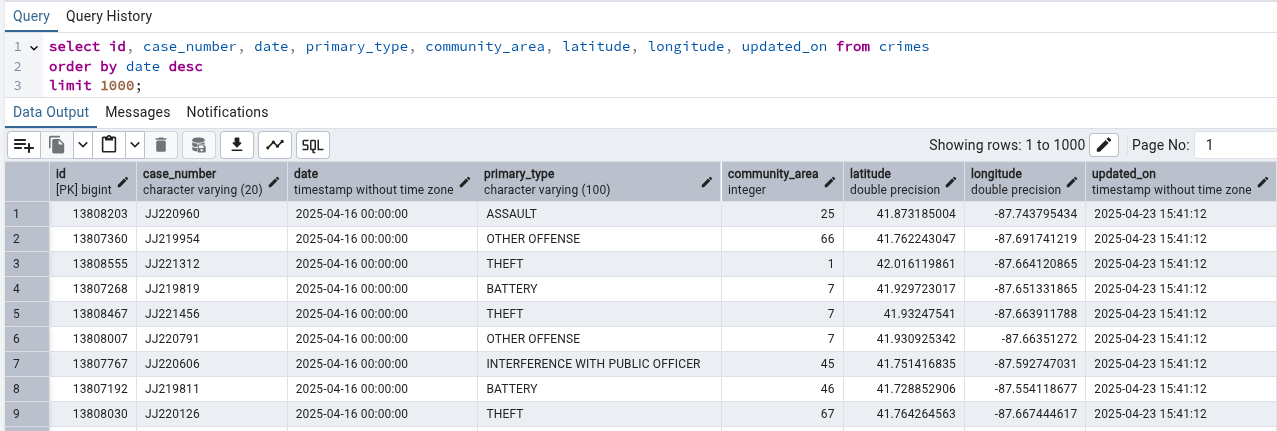
\includegraphics[width=1\textwidth]{figures/db_after_load.png}
    \caption{State of crimes table after latest load() operation}
    \label{fig:db_after_load}
\end{figure}

\section{Analysis \& Visualization}

\subsection*{Exploratory Data Analysis}
I performed exploratory data analysis after completing the ETL phase for the chicago crime data. This can be viewed in the ETL.ipynb notebook in the github repository. Few insights drawn from the analysis are listed below along with their supporting visualizations:





\begin{itemize}
    \item The overall crime count has been decreasing from 2001 to 2024 as shown in figure \ref{fig:crime_count_by_year}.
    \item There is seasonal trend present as shown by the figure \ref{fig:crime_count_by_month} where the number of crimes peaks around summer.
    \item From figure \ref{fig:crime_count_by_hour_of_day}, we can see that crime incidents clearly depend on the time of the day and number of crime peaks aroudn 12 PM.
    \item Theft is the most common crime type base on the figure \ref{fig:crime_count_by_crime_type} which shows the top 10 crime types by crime count.
    \item Street is the most common location where crime occurs based on the figure \ref{fig:crime_count_by_location} visualizing the top 10 location by crime count.
    \item Among the top 10 crime type by crime counts \texttt{Narcotics} has the highest arrest percentage as shown in figure \ref{fig:crime_type_by_arrest_proportion}.
    \item Figure \ref{fig:crime_distribution_in_2024} shows the distribution of crimes in 2024 in chicago.
\end{itemize}

% \begin{figure}[H]
%     \centering
%     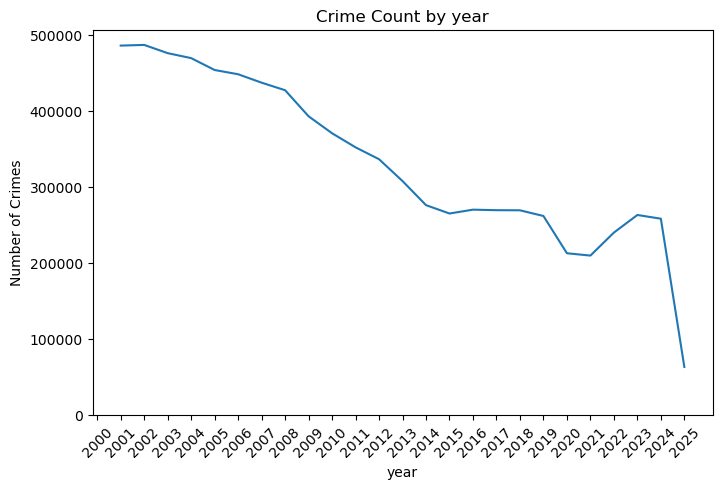
\includegraphics[width=0.45\textwidth]{figures/crime_count_by_year.png}
%     \caption{Overall crime count over the years}
%     \label{fig:crime_count_by_year.png}
% \end{figure}

% \begin{figure}[H]
%     \centering
%     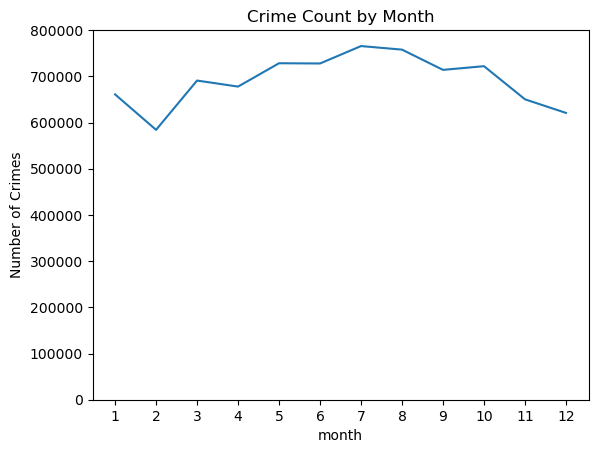
\includegraphics[width=0.45\textwidth]{figures/crime_count_by_month.png}
%     \caption{Seasonal trend of crime count}
%     \label{fig:crime_count_by_month}
% \end{figure}

% \begin{figure}[H]
%     \centering
%     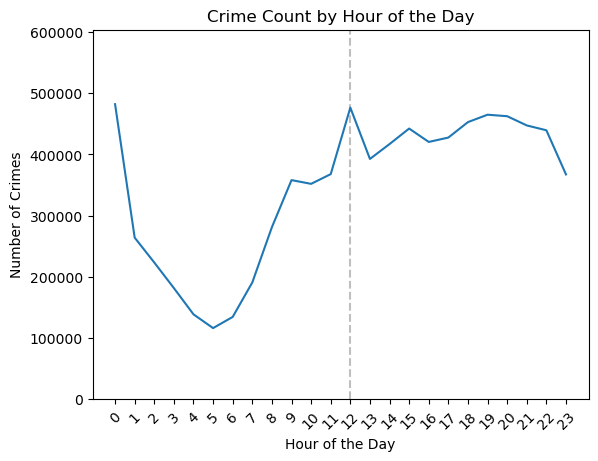
\includegraphics[width=0.45\textwidth]{figures/crime_count_by_hour_of_day.png}
%     \caption{Seasonal trend of crime count}
%     \label{fig:crime_count_by_hour_of_day}
% \end{figure}


% \begin{figure}[H]
%     \centering
%     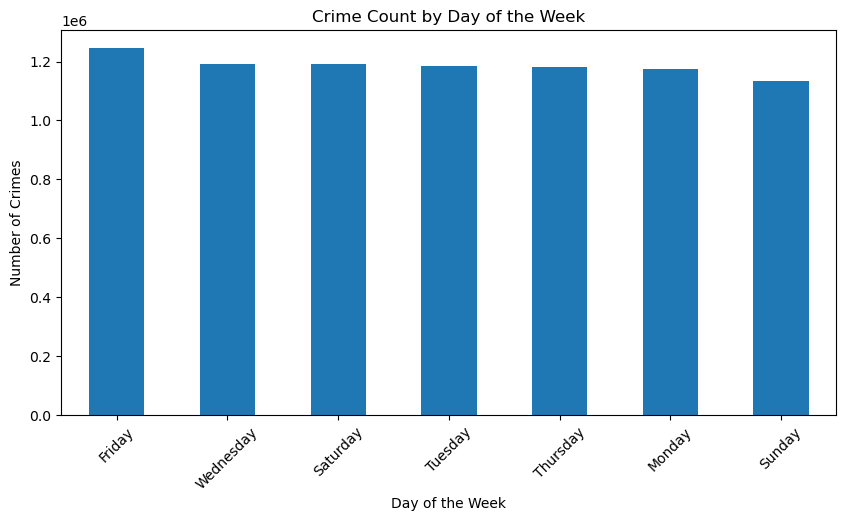
\includegraphics[width=0.45\textwidth]{figures/crime_count_by_day_of_the_week.png}
%     \caption{Seasonal trend of crime count}
%     \label{fig:crime_count_by_day_of_the_week}
% \end{figure}
\begin{figure}[H]
    \centering
    \begin{subfigure}[t]{0.49\textwidth}
        \centering
        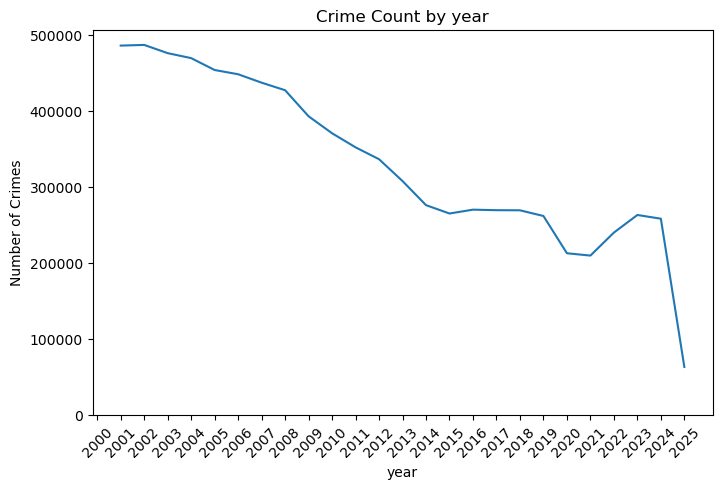
\includegraphics[width=\textwidth]{figures/crime_count_by_year.png}
        \caption{Overall crime count over the years}
        \label{fig:crime_count_by_year}
    \end{subfigure}
    \hfill
    \begin{subfigure}[t]{0.49\textwidth}
        \centering
        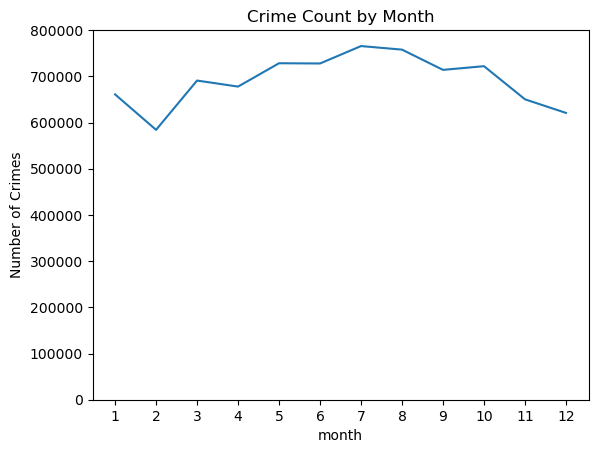
\includegraphics[width=\textwidth]{figures/crime_count_by_month.png}
        \caption{Seasonal trend of crime count}
        \label{fig:crime_count_by_month}
    \end{subfigure}
    \vskip\baselineskip
    \begin{subfigure}[t]{0.49\textwidth}
        \centering
        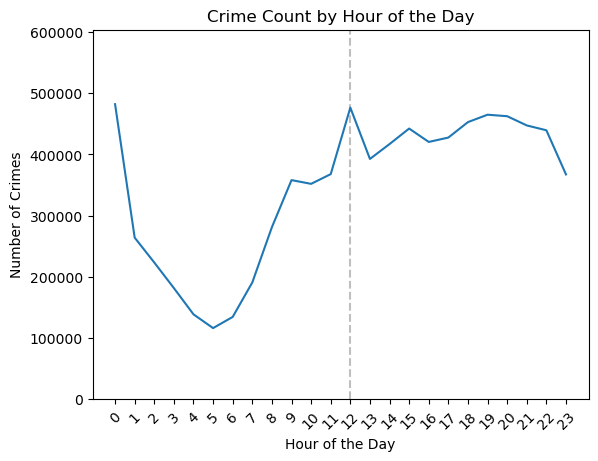
\includegraphics[width=\textwidth]{figures/crime_count_by_hour_of_day.png}
        \caption{Seasonal trend of crime count by hour of day}
        \label{fig:crime_count_by_hour_of_day}
    \end{subfigure}
    \hfill
    \begin{subfigure}[t]{0.49\textwidth}
        \centering
        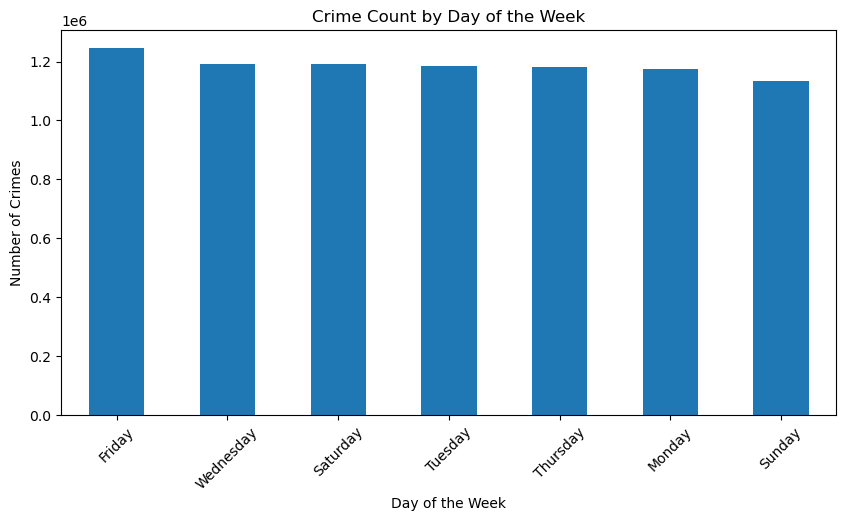
\includegraphics[width=\textwidth]{figures/crime_count_by_day_of_the_week.png}
        \caption{Seasonal trend of crime count by day of the week}
        \label{fig:crime_count_by_day_of_the_week}
    \end{subfigure}
    \caption{Crime count trends across different time dimensions}
    \label{fig:crime_trends}
\end{figure}

% \begin{figure}[H]
%     \centering
%     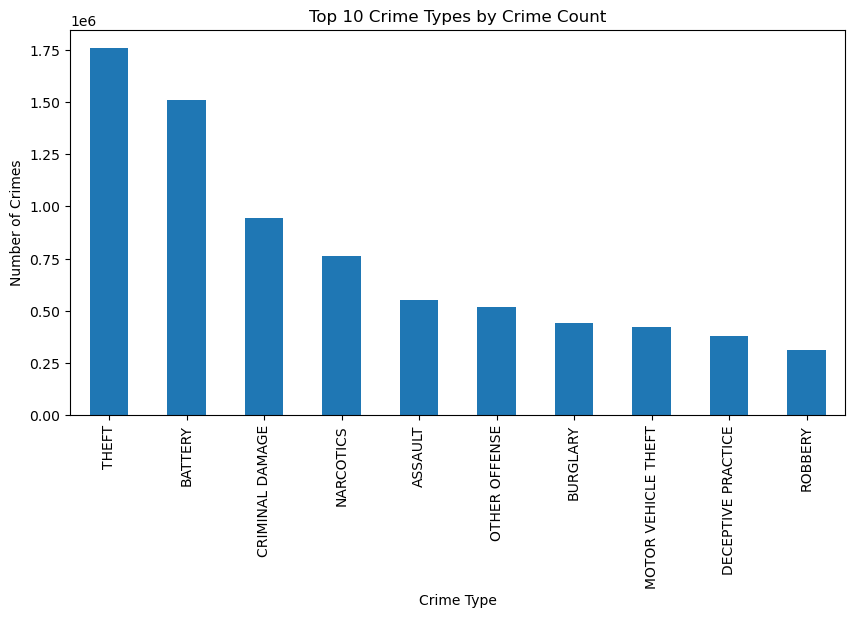
\includegraphics[width=0.7\textwidth]{figures/crime_count_by_crime_type.png}
%     \caption{Top 10 crime types by crime count}
%     \label{fig:crime_count_by_crime_type}
% \end{figure}
% \begin{figure}[H]
%     \centering
%     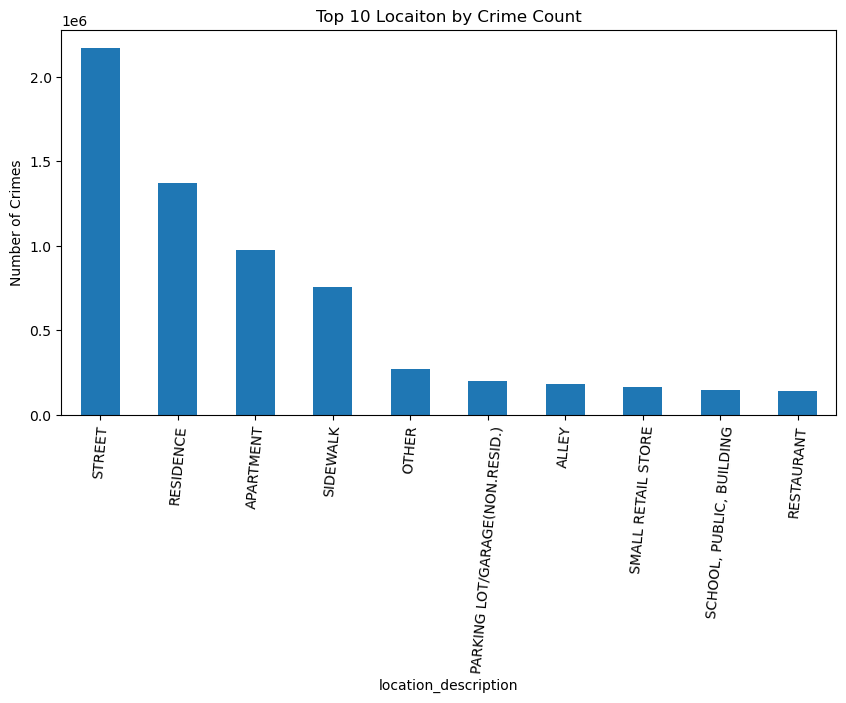
\includegraphics[width=0.7\textwidth]{figures/crime_count_by_location.png}
%     \caption{Top 10 locations by crime count}
%     \label{fig:crime_count_by_location}
% \end{figure}
% \begin{figure}[H]
%     \centering
%     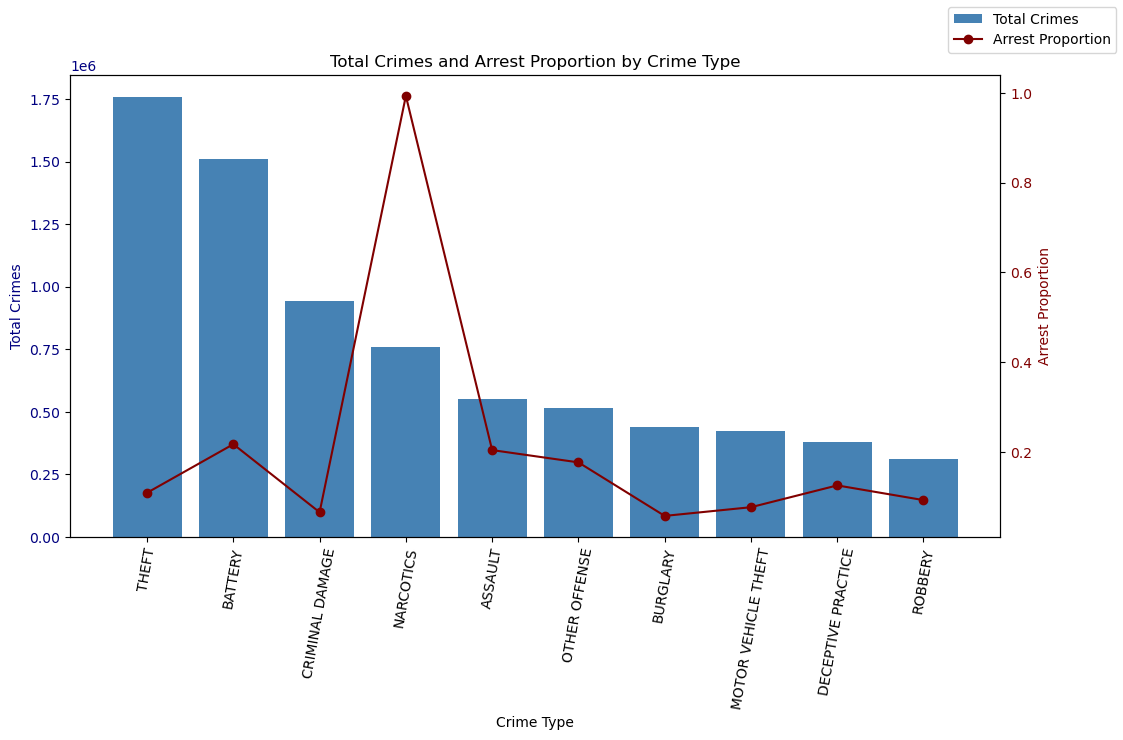
\includegraphics[width=0.7\textwidth]{figures/crime_type_by_arrest_proportion.png}
%     \caption{Arrest percentage by crime type}
%     \label{fig:crime_type_by_arrest_proportion}
% \end{figure}    
% \begin{figure}[H]
%     \centering
%     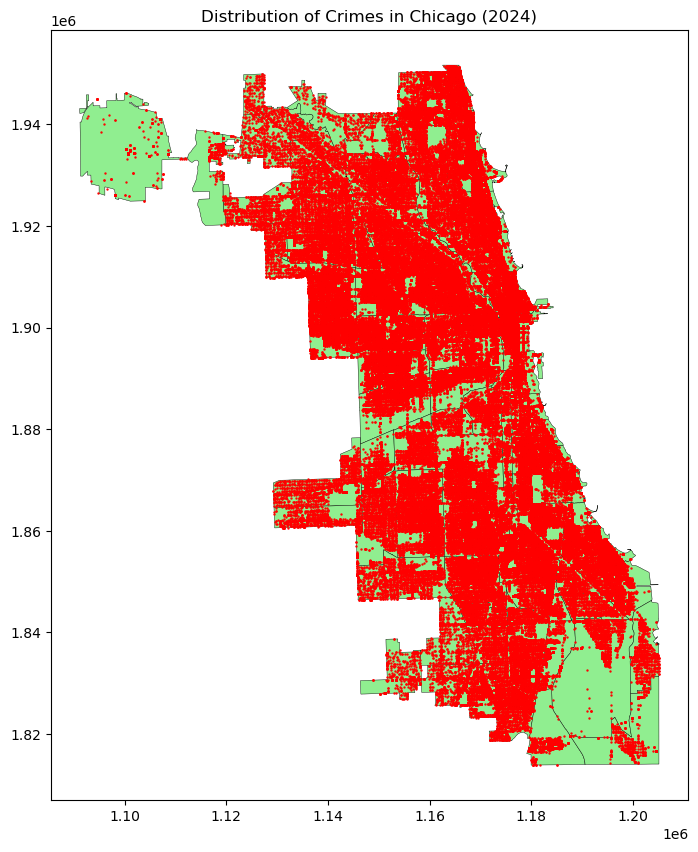
\includegraphics[width=0.5\textwidth]{figures/crime_distribution_in_2024.png}
%     \caption{Distribution of crime incidents in 2024}
%     \label{fig:crime_distribution_in_2024}
% \end{figure}    

\begin{figure}[H]
    \centering
    \begin{subfigure}[t]{0.49\textwidth}
        \centering
        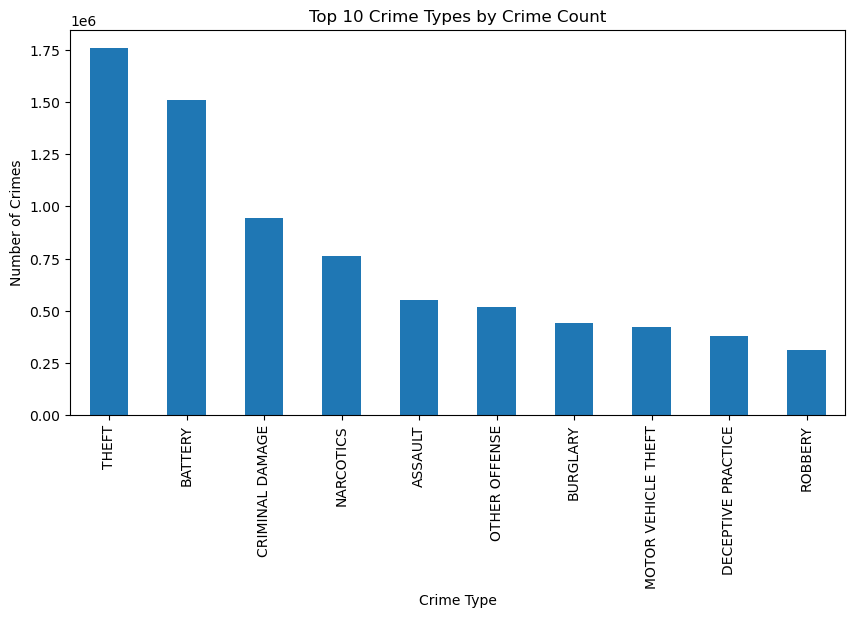
\includegraphics[width=\textwidth]{figures/crime_count_by_crime_type.png}
        \caption{Top 10 crime types by crime count}
        \label{fig:crime_count_by_crime_type}
    \end{subfigure}
    \hfill
    \begin{subfigure}[t]{0.49\textwidth}
        \centering
        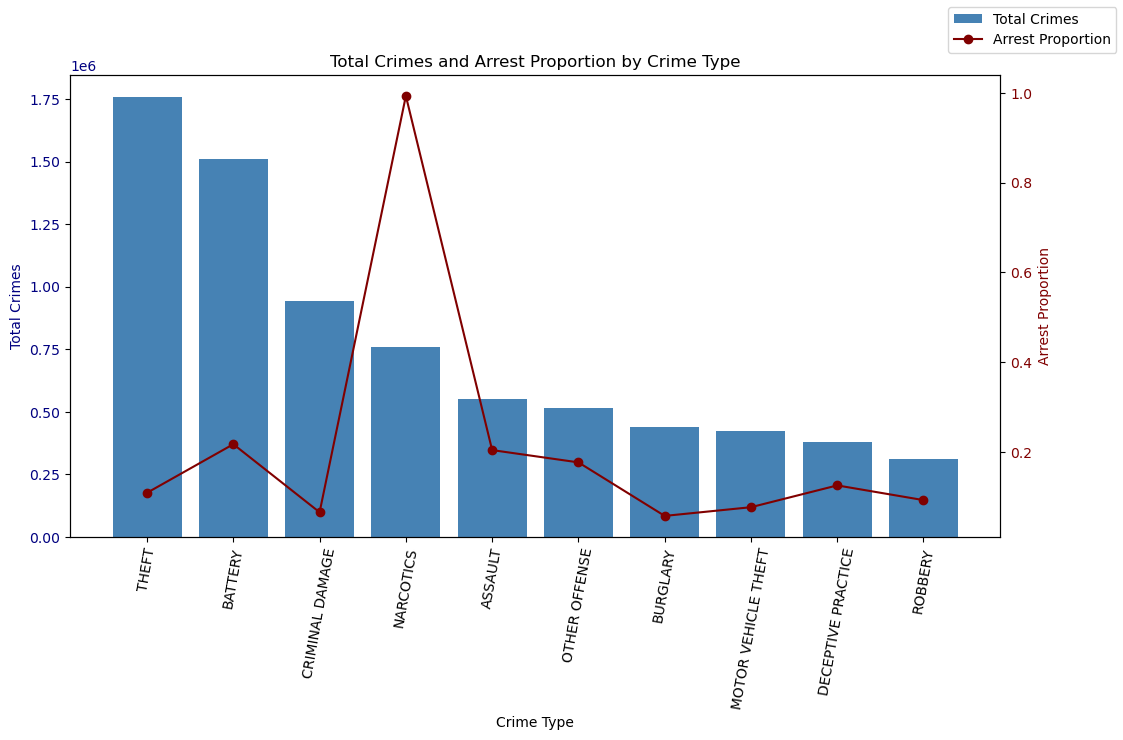
\includegraphics[width=\textwidth]{figures/crime_type_by_arrest_proportion.png}
        \caption{Arrest percentage by crime type}
        \label{fig:crime_type_by_arrest_proportion}
    \end{subfigure}
   
    \vskip\baselineskip
    \begin{subfigure}[t]{0.49\textwidth}
        \centering
        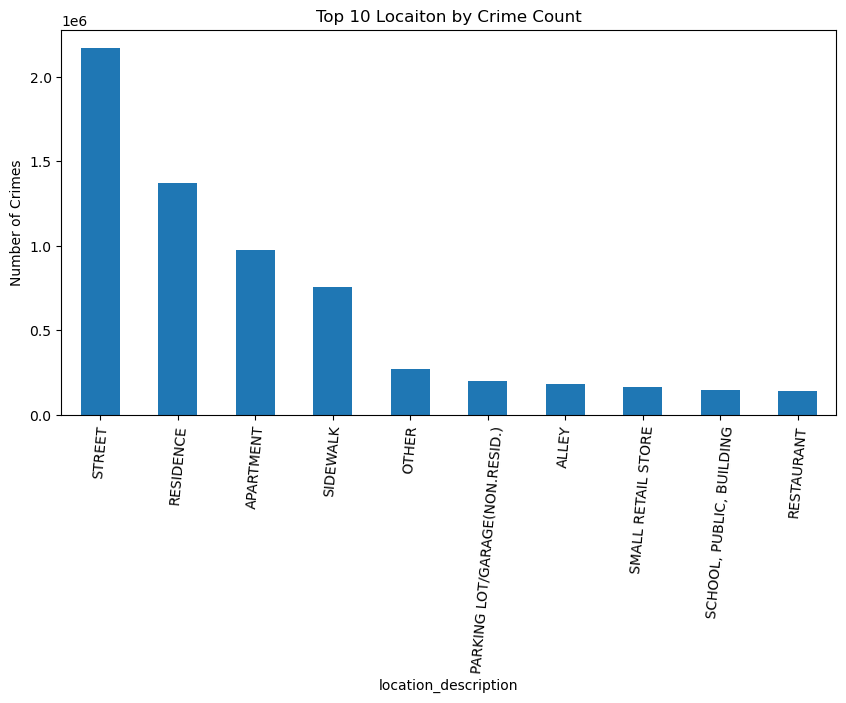
\includegraphics[width=\textwidth]{figures/crime_count_by_location.png}
        \caption{Top 10 locations by crime count}
        \label{fig:crime_count_by_location}
    \end{subfigure}
    \hfill
    \begin{subfigure}[t]{0.49\textwidth}
        \centering
        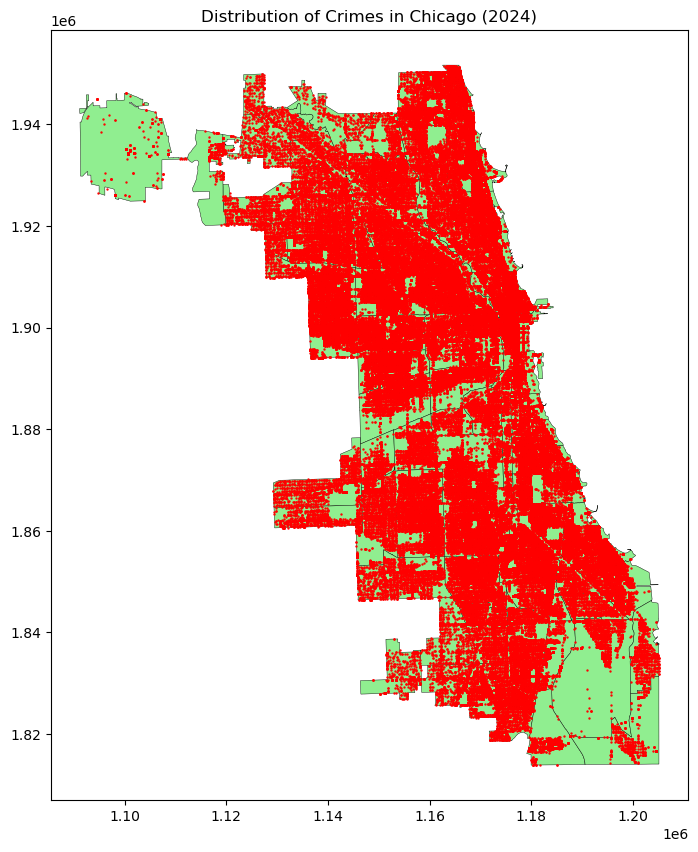
\includegraphics[width=\textwidth]{figures/crime_distribution_in_2024.png}
        \caption{Distribution of crime incidents in 2024}
        \label{fig:crime_distribution_in_2024}
    \end{subfigure}
    \caption{Crime data visualizations: crime types, locations, arrest proportions, and 2024 distribution}
    \label{fig:crime_data_visualizations}
\end{figure}



\section{Looker Studio Integration}

To make the transformed and enriched crime data easily consumable, I connected the PostgreSQL database (hosted on Aiven) to Google Looker Studio to create dynamic visual dashboards. The dashboard allows users to explore crime trends, types, and locations interactively. It can be accessed from this link: \href{https://lookerstudio.google.com/reporting/73440c10-3d68-47ac-b150-026b80c468c0}{here}.

\begin{figure}[h!]
    \centering
    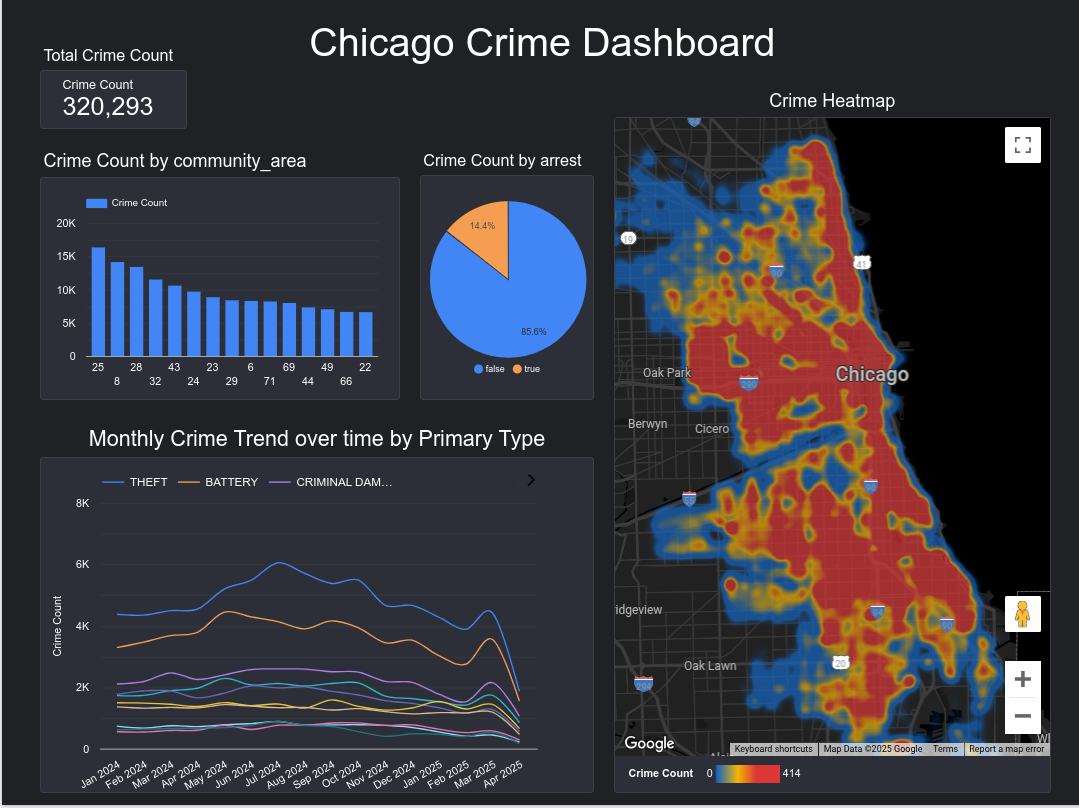
\includegraphics[width=0.9\textwidth]{figures/looker_dashboard.png}
    \caption{Looker Studio Geo Map showing crime intensity by location}
    \label{fig:looker_dashboard}
\end{figure}

\subsection*{Data Source Configuration}
Initially, I attempted to expose my local PostgreSQL server to Looker Studio using Ngrok. However, this approach was abandoned for the following reasons:
\begin{itemize}
    \item Public exposure of local resources is not secure for production
    \item Requires a continuously running local machine
    \item Ngrok tunnels on the free tier expire frequently
\end{itemize}

Instead, I setup the database in Aiven’s managed PostgreSQL instance. This cloud-hosted database ensures consistent availability and does not depend on my local infrastructure.

\subsection*{Creating the Connection}
\begin{itemize}
    \item In Looker Studio, I selected the “PostgreSQL” connector
    \item I entered the Aiven host, port, user, and password 
    \item I chose views such as \texttt{crimes\_by\_month}, \texttt{crimes\_by\_location}, and \texttt{crimes\_by\_type} to power the dashboard
\end{itemize}

\subsection*{Enabling Geospatial Visualization}
Looker Studio requires a single “Location” field for geo maps. Since my data stores latitude and longitude separately, I created a calculated field:

\begin{lstlisting}[language=SQL, caption={Looker Studio calculated field for geo mapping}]
CONCAT(latitude , ",",longitude)
\end{lstlisting}

This field was used as the “Location” dimension in geo maps to visualize hotspots of criminal activity.



\section{Monitoring and Logging}

\subsection*{Systemd Status Monitoring}
Airflow was configured to run as a systemd service, making it easy to check the status at any time:

\begin{lstlisting}[language=bash]
sudo systemctl status airflow
\end{lstlisting}

If Airflow or the system is restarted, the scheduler and webserver start automatically in the background.

\subsection*{Airflow Logs}
Each task logs detailed output visible from the Airflow UI or saved to disk under the \texttt{logs/} directory. These logs include:
\begin{itemize}
    \item Retry attempts
    \item Record counts
    \item Timestamps
    \item Error tracebacks
\end{itemize}

\subsection*{Audit Logs}
Transformation and loading steps generate CSV files for any dropped or failed records:
\begin{itemize}
    \item \texttt{audit\_missing\_drops\_\{timestamp\}.csv}
    \item \texttt{audit\_duplicate\_drops\_\{timestamp\}.csv}
    \item \texttt{failed\_batch\_\{n\}\_\{timestamp\}.csv}
\end{itemize}

These files are timestamped and saved locally, allowing me to inspect issues post-run without affecting the main pipeline.

\subsection*{Resource Monitoring}
Because the VM is a Google Cloud e2-micro instance, I used \texttt{htop} to monitor CPU and memory usage. Since the system only has 1GB of RAM, it frequently crashed when I tried to ssh into it through vscode, so, I created a 4GB of swap space to mitigate those crashes. The pipeline is optimized for low memory usage by processing data in batches, avoiding unnecessary copies, and running on minimal infrastructure.

\begin{figure}[h!]
    \centering
    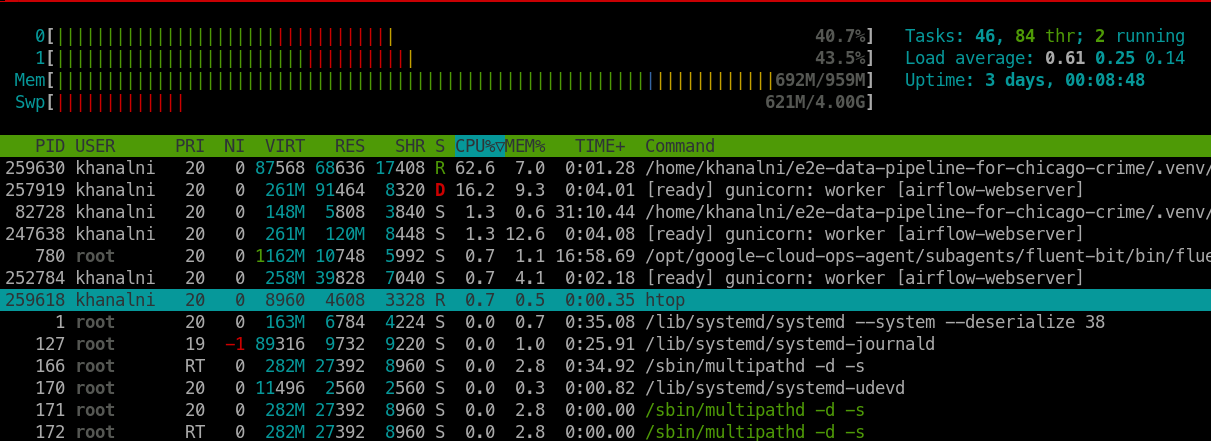
\includegraphics[width=0.9\textwidth]{figures/htop_during_load.png}
    \caption{Resource usage during load task, monitored using \texttt{htop}}
    \label{fig:htop}
\end{figure}

\subsection*{Accessing the Airflow Dashboard Securely}

Since the Airflow webserver was running on port 8080 inside a remote VM (Google Cloud), I used SSH port forwarding to securely access the dashboard from my local browser without exposing it to the public internet.

The command I used was:

% \begin{lstlisting}[language=bash]
\texttt{ssh $-$L 8080:localhost:8080 khanalni@34.56.242.64}
% \end{lstlisting}

This forwards the VM’s port \texttt{8080} to my local machine’s port \texttt{8080}, allowing me to view the dashboard by navigating to \texttt{http://localhost:8080} in my browser.

\begin{figure}[h!]
    \centering
    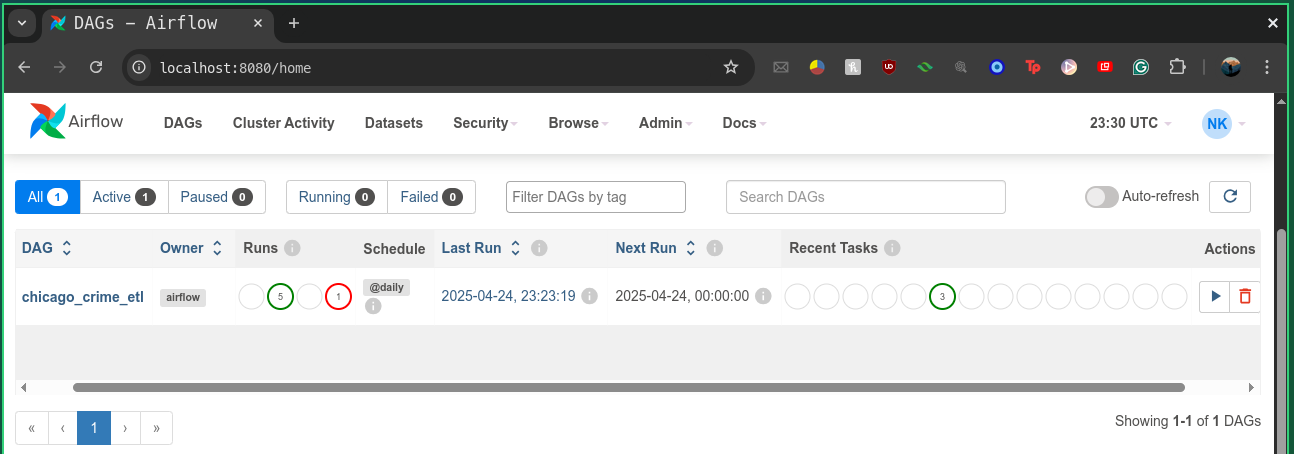
\includegraphics[width=0.9\textwidth]{figures/airflow_dashboard_ui.png}
    \caption{Airflow dashboard running remotely, accessed via SSH port forwarding}
    \label{fig:airflow_ui}
\end{figure}

Using SSH port forwarding avoided the need for opening firewall rules or exposing the webserver publicly, which is particularly important for VMs without HTTPS or basic authentication.


\section{Security and Secrets Management}

In this project, several sensitive credentials are used, including:
\begin{itemize}
    \item PostgreSQL database credentials for the Aiven instance
    \item API tokens for the Socrata open data platform
    \item Airflow configurations that may store DAG execution metadata
\end{itemize}

To avoid hardcoding secrets in source files, I followed best practices for managing credentials securely.

\subsection*{Using \texttt{.env} Files}
All sensitive information was stored in a \texttt{.env} file at the root of the project directory. This file is read at runtime using the \texttt{python-dotenv} library.

\begin{lstlisting}[language=bash]
# .env (never committed to version control)
DB_HOST=db.aiven.io
DB_USER=myuser
DB_PASS=secure_password_here
DB_NAME=crime_data
APP_TOKEN=my_socrata_token
\end{lstlisting}

In Python, these values were loaded as:

\begin{lstlisting}[language=python]
from dotenv import load_dotenv
import os

load_dotenv()

db_config = {
    "host": os.getenv("DB_HOST"),
    "port": os.getenv("DB_PORT"),
    "dbname": os.getenv("DB_NAME"),
    "user": os.getenv("DB_USER"),
    "password": os.getenv("DB_PASS")
}

app_token = os.getenv("APP_TOKEN")
\end{lstlisting}

This ensures that secrets are never exposed in the codebase, nor are they accidentally committed to GitHub.

\subsection*{Version Control}
The \texttt{.env} file and other sensitive scripts were added to \texttt{.gitignore} to prevent accidental inclusion in the repository.

\begin{lstlisting}[language=bash]
# .gitignore
.env
*.log
*.csv
logs/
\end{lstlisting}

\subsection*{Cloud Credentials}
For the Aiven PostgreSQL database:
\begin{itemize}
    \item A dedicated user with limited privileges was created
    \item SSL was enabled by default
    \item The connection string was never exposed publicly
\end{itemize}

\subsection*{Airflow Configuration}
For local development and production automation:
\begin{itemize}
    \item Airflow connections and variables were avoided in plaintext
\end{itemize}
   
These practices helped ensure that the pipeline could run securely without exposing critical credentials during deployment, development, or daily automation.

\section{Conclusion and Future Work}

This project was able to deliver a fully functional and automated ETL pipeline for Chicago crime data processing. The pipeline was designed for reliability, scalability, and ease of maintenance when running on low infrastructure. It includes real-time API extraction, intensive transformation with spatial enrichment, batch-optimized PostgreSQL loading, and visualization with Looker Studio — all orchestrated with Airflow on a micro GCP VM.

\subsection*{Key Accomplishments}
\begin{itemize}
    \item Built a modular ETL framework using Python, with well-separated concerns (extract, transform, load)
    \item Implemented robust exception handling and audit logging to ensure traceability
    \item Enabled geospatial enrichment of missing fields via shapefile-based joins
    \item Migrated from local development to a fully cloud-hosted pipeline with no dependency on local resources
    \item Used Airflow for orchestration, systemd for automation, and Looker Studio for visualization
\end{itemize}

\subsection*{Lessons Learned}
\begin{itemize}
    \item Development tools like \texttt{ngrok} are useful for prototyping but unsuited for production pipelines
    \item Memory-efficient techniques such as chunked CSV processing and in-place DataFrame transformations are essential on constrained VMs
    \item Investing in early error handling and audit logging dramatically reduces debugging overhead
    \item Choosing managed services like Aiven allows for a highly available system with minimal DevOps effort
\end{itemize}

\subsection*{Future Enhancements}
\begin{itemize}
    \item \textbf{Dockerize the pipeline}: Containerize the ETL pipeline and run it with Docker Compose or Kubernetes for portability and environment isolation
    \item \textbf{Slack/Email alerts}: Configure Airflow to send failure notifications to Slack or email for real-time monitoring
    \item \textbf{Add support for other cities}: Generalize the pipeline to support similar datasets from other U.S. cities
\end{itemize}

\vspace{0.5cm}
\noindent The result is a cloud-native, resource-efficient data pipeline that can grow to support more complex workflows and richer analytics in the future.


% \section*{References}
\addcontentsline{toc}{section}{References}
% \nocite{pandas,airflow,geopandas,sodapy}
\nocite{*}
\bibliographystyle{plain}
\bibliography{references}

\end{document}